% lecture14.tex — Orientation

\section{Orientation}

\begin{definition}{Equivalently Oriented Bases}{equiv-oriented-bases}
    Suppose $V$ is a finite dimensional real vector space, and $\beta = \{v_1, \ldots, v_k\}$ and $\beta' = \{v_1', \ldots, v_k'\}$ are two ordered bases. Then there is a unique linear isomorphism $A \colon V \to V$ such that $\beta' = A\beta$. We say $\beta$ and $\beta'$ are \emph{equivalently oriented} if $\det A > 0$.
\end{definition}

This gives an equivalence relation on the set of all ordered bases of $V$, and there are exactly two equivalence classes ($\operatorname{GL}(V)$ has 2 components).

\begin{definition}{Orientation of a Vector Space}{orientation-vector-space}
    An \emph{orientation} of $V$ is a choice of one of those two equivalence classes.
\end{definition}

An orientation induces a sign ($+$ or $-$) on any ordered basis of $V$.

($*$ When $V = 0$, we separately define its orientation to be a choice of a sign $\in \{+, -\}$.)

\begin{example}{Orientation of $\R^2$}{orientation-R2}
    Say, $V = \R^2$ and choose $[(e_1, e_2)]$ for the orientation. Then counterclockwise bases are positively oriented, while clockwise bases are negatively oriented.
\end{example}

\begin{center}
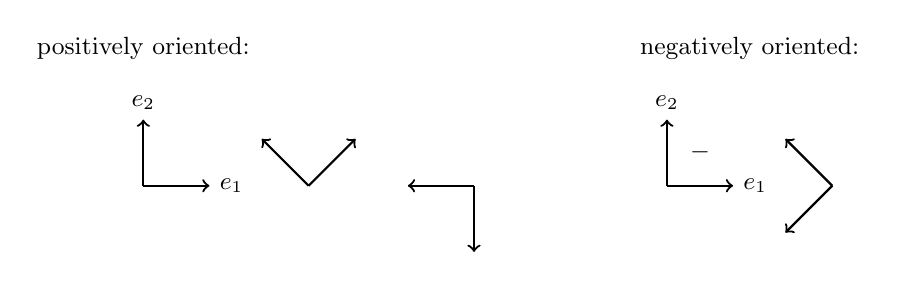
\begin{tikzpicture}[scale=0.7]
    % Positively oriented examples
    \node at (0,2.5) {\small positively oriented:};
    % Standard basis
    \draw[->,thick] (0,0) -- (1.2,0) node[right] {\small $e_1$};
    \draw[->,thick] (0,0) -- (0,1.2) node[above] {\small $e_2$};
    % Rotated
    \begin{scope}[xshift=3cm]
        \draw[->,thick] (0,0) -- (0.85,0.85);
        \draw[->,thick] (0,0) -- (-0.85,0.85);
    \end{scope}
    % Another
    \begin{scope}[xshift=6cm]
        \draw[->,thick] (0,0) -- (-1.2,0);
        \draw[->,thick] (0,0) -- (0,-1.2);
    \end{scope}
    % Negatively oriented examples
    \node at (11,2.5) {\small negatively oriented:};
    \begin{scope}[xshift=9.5cm]
        \draw[->,thick] (0,0) -- (0,1.2) node[above] {\small $e_2$};
        \draw[->,thick] (0,0) -- (1.2,0) node[right] {\small $e_1$};
        \node at (0.6,0.6) {\small $-$};
    \end{scope}
    \begin{scope}[xshift=12.5cm]
        \draw[->,thick] (0,0) -- (-0.85,0.85);
        \draw[->,thick] (0,0) -- (-0.85,-0.85);
    \end{scope}
\end{tikzpicture}
\end{center}

Note, if $V$ and $W$ are oriented real vector spaces of the same dimension, then any isomorphism $A \colon V \to W$ either \emph{preserves} or \emph{reverses} orientation.

\subsection{Orientation of Manifolds}

\begin{definition}{Orientation of a Manifold}{orientation-manifold}
    An \emph{orientation} of $M$, a manifold with boundary, is a smooth choice of orientations for all tangent spaces $T_p M$.

    That is, around each $p \in M$, there is a local parametrization $h \colon U \to M$, $U \subset H^m \subset \R^m$, such that $dh_u \colon T_u U \cong \R^m \to T_{h(u)} M$ preserves orientation for all $u \in U$, where $\R^m$ is given the standard orientation $[(e_1, \ldots, e_m)]$.
\end{definition}

A smooth map between oriented manifolds of the same dimension whose derivative preserves orientations at every point is called an \emph{orientation-preserving map}.

\begin{example}{Non-Orientable Manifolds}{non-orientable}
    Not all manifolds can be oriented! The M\"obius band is not orientable.
\end{example}

\begin{center}
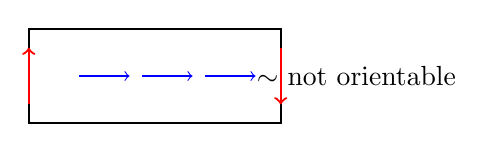
\begin{tikzpicture}[scale=0.8]
    % Mobius band as rectangle with identification
    \draw[thick] (0,0) rectangle (4,1.5);
    % Arrows on left side (upward)
    \draw[->,thick,red] (0,0.3) -- (0,1.2);
    % Arrows on right side (downward — reversed!)
    \draw[->,thick,red] (4,1.2) -- (4,0.3);
    % Orientation arrows along the band
    \draw[->,blue] (0.8,0.75) -- (1.6,0.75);
    \draw[->,blue] (1.8,0.75) -- (2.6,0.75);
    \draw[->,blue] (2.8,0.75) -- (3.6,0.75);
    \node at (5.2,0.75) {$\sim$ not orientable};
\end{tikzpicture}
\end{center}

\begin{example}{Orientable Manifolds}{orientable-examples}
    $T^2$ (torus) and $S^2$ (sphere) are orientable.
\end{example}

\begin{center}
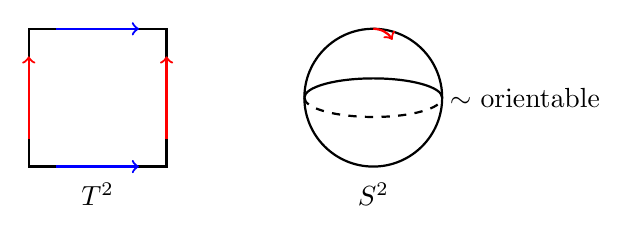
\begin{tikzpicture}[scale=0.7]
    % Torus as rectangle with identifications
    \draw[thick] (0,0) rectangle (2.5,2.5);
    \draw[->,thick,red] (0,0.5) -- (0,2);
    \draw[->,thick,red] (2.5,0.5) -- (2.5,2);
    \draw[->,thick,blue] (0.5,0) -- (2,0);
    \draw[->,thick,blue] (0.5,2.5) -- (2,2.5);
    \node at (1.25,-0.5) {$T^2$};
    % Sphere
    \begin{scope}[xshift=5cm]
        \draw[thick] (1.25,1.25) circle (1.25);
        \draw[thick,dashed] (0,1.25) arc(180:360:1.25 and 0.35);
        \draw[thick] (0,1.25) arc(180:0:1.25 and 0.35);
        % Orientation arrow
        \draw[->,thick,red] (1.25,2.5) arc(90:30:0.4);
        \node at (1.25,-0.5) {$S^2$};
    \end{scope}
    \node at (9,1.25) {$\sim$ orientable};
\end{tikzpicture}
\end{center}

\begin{proposition}{Two Orientations}{two-orientations}
    A connected, orientable manifold with boundary admits exactly two orientations.
\end{proposition}

\begin{proof}
    The set of points at which two orientations agree and the set where they disagree are both open. Consequently, two orientations of a connected manifold are either identical or opposite.
\end{proof}

\subsection{Product and Boundary Orientations}

\begin{remark}{Product and Boundary Orientations}{product-boundary-orientations}
    \begin{itemize}
        \item The product $M \times N$ of two oriented manifolds (where one of them is boundaryless) acquires a \emph{product orientation}, for if $\alpha$ and $\beta$ are ordered bases for $T_p M$ and $T_q N$, then $(\alpha \times 0, 0 \times \beta)$ is an ordered basis for $T_{(p,q)}(M \times N) \cong T_p M \times T_q N$.

        \item An orientation of $M$ induces a \emph{boundary orientation} on $\partial M$; this can be done by declaring the sign of any ordered basis $\beta = \{v_1, \ldots, v_{m-1}\}$ of $T_p(\partial M)$ to be the sign of the ordered basis $\{n_p, v_1, \ldots, v_{m-1}\}$, where $n_p$ is the outward unit normal at $p$.
    \end{itemize}
\end{remark}

\begin{example}{Boundary Orientation of $I \times M$}{boundary-orientation-cylinder}
    For the cylinder $I \times M$, the boundary orientation gives $\partial(I \times M) = M_1 - M_0$, where $M_0$ and $M_1$ have opposite orientations.
\end{example}

\begin{center}
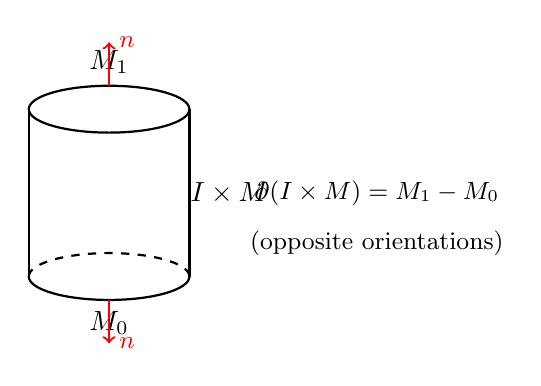
\begin{tikzpicture}[scale=0.85]
    % Cylinder
    \draw[thick] (-1.2,0) -- (-1.2,2.5);
    \draw[thick] (1.2,0) -- (1.2,2.5);
    % Bottom circle M_0
    \draw[thick] (-1.2,0) arc(180:360:1.2 and 0.35);
    \draw[thick,dashed] (-1.2,0) arc(180:0:1.2 and 0.35);
    % Top circle M_1
    \draw[thick] (-1.2,2.5) arc(180:360:1.2 and 0.35);
    \draw[thick] (-1.2,2.5) arc(180:0:1.2 and 0.35);
    % Labels
    \node at (0,-0.7) {$M_0$};
    \node at (0,3.2) {$M_1$};
    \node at (1.8,1.25) {$I \times M$};
    % Outward normals
    \draw[->,thick,red] (0,2.85) -- (0,3.5) node[right] {\small $n$};
    \draw[->,thick,red] (0,-0.35) -- (0,-1) node[right] {\small $n$};
    % Orientation note
    \node at (4,1.25) {\small $\partial(I \times M) = M_1 - M_0$};
    \node at (4,0.5) {\small (opposite orientations)};
\end{tikzpicture}
\end{center}

\subsection{Orienting Preimages}

If $V = V_1 \oplus V_2$, the orientations on any two of $V$, $V_1$, $V_2$ induce a \emph{direct sum orientation} on the third. (The ordering of summands is important!)

We can use this to orient $f^{-1}(P) =: Q$ if $f \colon M \to N$, $f \pitchfork P$, $f|_{\partial M} \pitchfork P$, and $M$, $N$, $P$ are all oriented.

Let $N_x(Q; M)$ be the orthogonal complement of $T_x Q$ in $T_x M$, so that
\[
    T_x M = N_x(Q; M) \oplus T_x Q.
\]
By transversality,
\[
    T_y N = df_x(N_x(Q; M)) \oplus T_y P,
\]
which gives an orientation on $T_x Q$!

\begin{proposition}{Boundary of Preimage}{boundary-preimage-orientation}
    $\partial f^{-1}(P) = (-1)^{\codim P} (f|_{\partial M})^{-1}(P)$.
\end{proposition}

\begin{proof}[Proof sketch]
    $T_x M = N_x(Q; M) \oplus \R \cdot n_x \oplus T_x(\partial Q) = \R \cdot n_x \oplus N_x(Q; M) \oplus T_x((f|_{\partial M})^{-1}(P))$, so the orientations differ by $(-1)^{\codim Q} = (-1)^{\codim P}$.
\end{proof}
